\subsection{Three-Dimensional Data}\label{sec:results3d}
\begin{figure*}[t]
\centering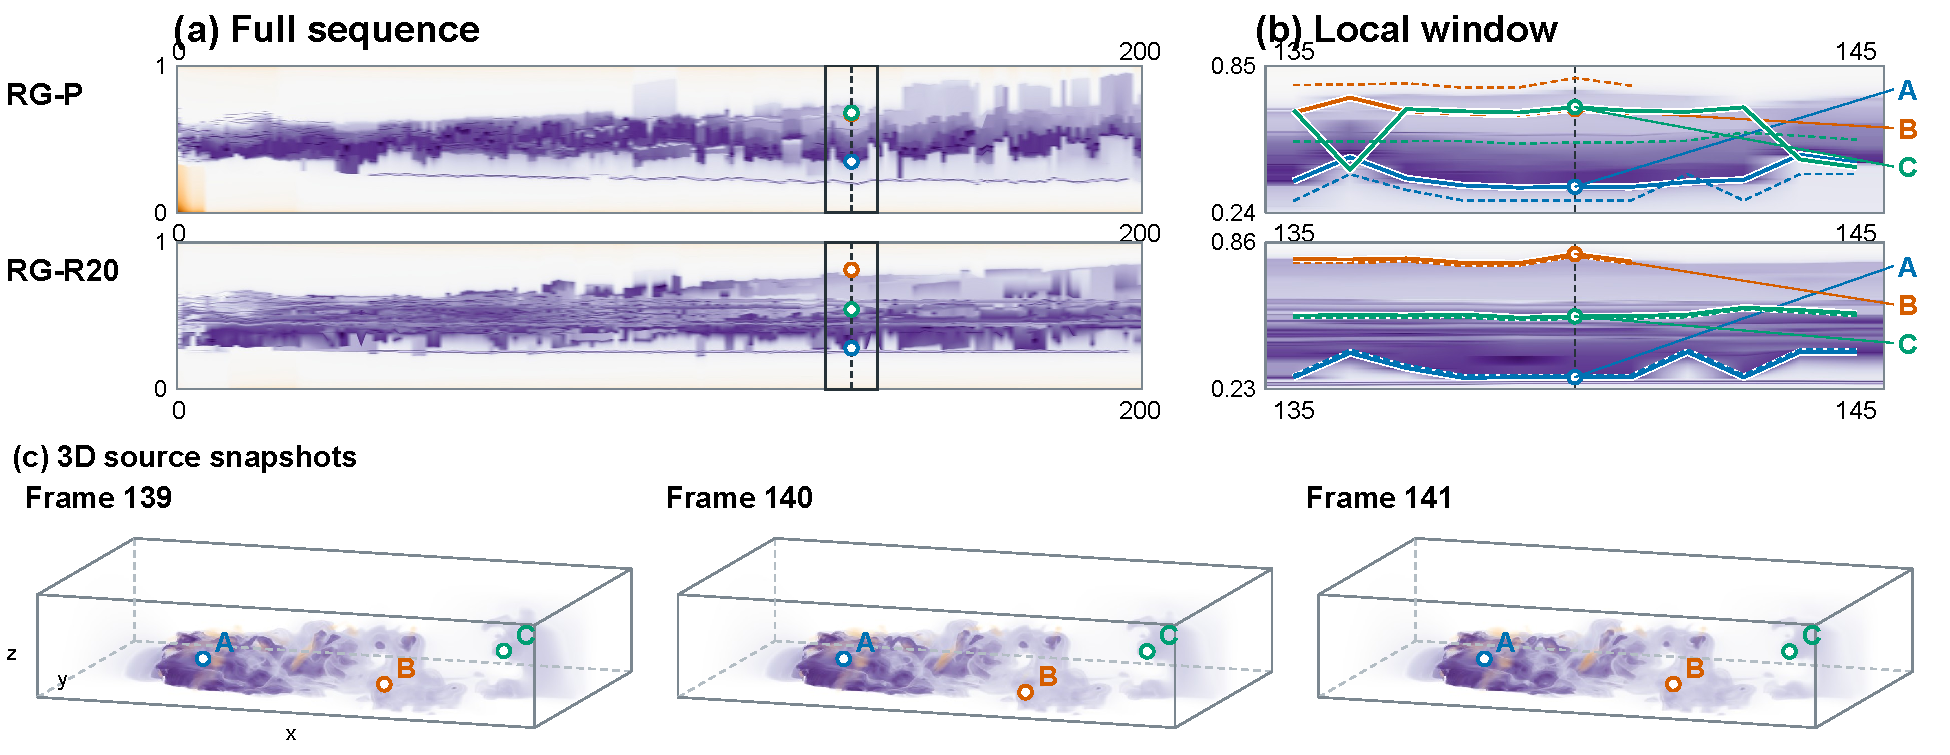
\includegraphics[width=\textwidth]{figures/Fig10.pdf}
\caption{Tangaroa: RG-MTM-P/R20 across all 201 original-grid fields (a), the local window 135--145 (b), and full-volume views at frames 139--141 (c). Tracks $A=432$, $B=462$, $C=388$ link saved anchors, dashed references, and true three-dimensional extrema. The common orthographic camera and domain frames preserve spatial context. The retained purple--white--orange speed transfer function uses $[0,2]$. At frame 140, P/R maximum displacement is 14.76\%/1.02\%, with 13.75\% actual R NMLE. Full baseline panels and rendering details are in Supplement S6, S8, and S10. Temporal colour transitions use display interpolation only; saved frames, anchors, and evaluation samples are unchanged.}
\label{fig:volume}
\end{figure*}

\begin{figure*}[t]
\centering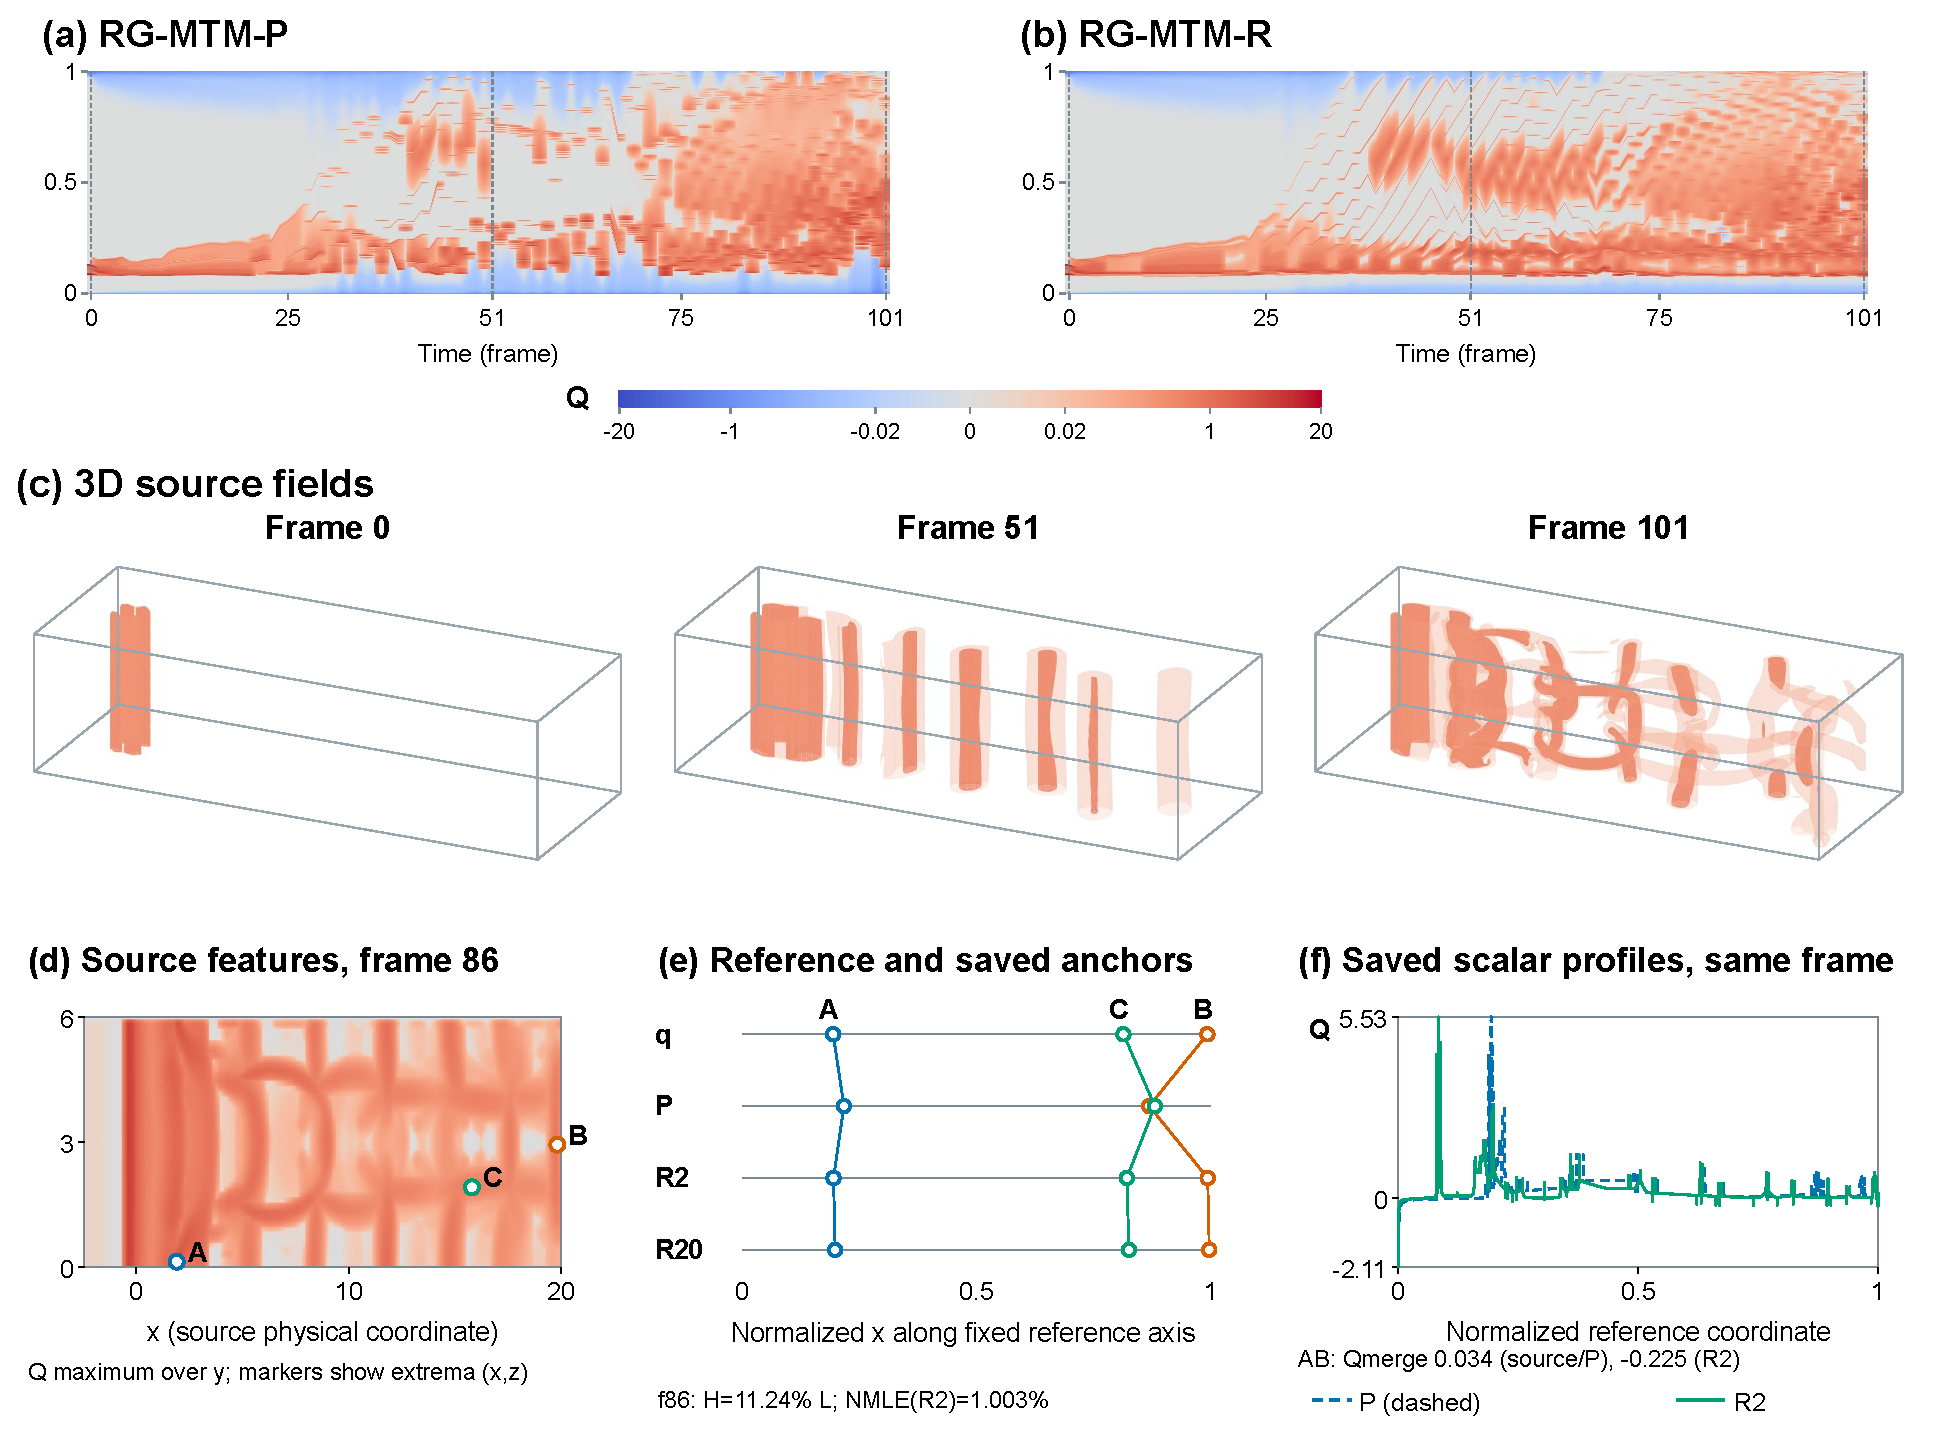
\includegraphics[width=\textwidth]{figures/Fig11.pdf}
\caption{Cylinder: RG-MTM-P (a) and R20 (b) for all 102 original-grid three-dimensional $Q$ fields, with source isosurfaces at frames 0, 51, and 101 (c). The maps use normalized physical $x$ reference position; vertical guides locate the source views. Their common symmetric-log colour scale is linear within $\pm0.02$. Isosurfaces at $Q=0.1$ (translucent) and $0.5$ (solid) share physical aspect, camera, and domain frame. Source views precede persistence simplification; maps use the common simplified inputs. Full TMTM/R2 panels and rendering details are in Supplement S9--S10. Panels (d)--(f) link a median-criterion selected conflict at frame 86 to its source features, continuous anchors and complete P/R2 profiles. Maximum displacement changes from 12.40\% to 1.17\% of reference extent, with 1.003\% R2 NMLE. The local case is descriptive; full-sequence scores remain in the common tables. The source projection in (d) uses bilinear display reconstruction with exact original cell centers. Temporal colour transitions use display interpolation only; saved frames, anchors, and evaluation samples are unchanged.}
\label{fig:cylinder}
\end{figure*}

\paragraph{Completed volumetric baseline and geometry comparison.}
All 303 volumetric inputs now have native ST-MTM layouts and the same SNS/TW/TD evaluation as the planar data (Table~\ref{tab:tradeoff}). On Tangaroa, ST-MTM reduces SNS from TMTM's 0.5255 to 0.1655 and increases TW from 0.6701 to 0.8137. Its NROE is 21.34\%, compared with P's 9.61\% and R20's 0.019\%, while its TD is 138.55 versus TMTM's 64.86 and R20's 39.71. Relative-distance quality, reference alignment and temporal stability therefore give different rankings on this sequence.

On Cylinder, ST-MTM reduces TMTM's NROE from 26.62\% to 17.77\%, SNS from 0.2956 to 0.1346 and TD from 85.03 to 43.17. R20 has lower NROE (0.084\%), SNS (0.0399) and TD (29.11), but slightly lower TW (0.8912 versus ST-MTM's 0.8989) and nonzero merge-level cost. ST-MTM makes 4730/6755 Tangaroa and 1469/3196 Cylinder motion errors under each dataset's retained threshold protocol; P/R20 make 3697/2060 and 1191/605, respectively. These are within-dataset geometric proxies, not pooled accuracies. All new ST-MTM profiles preserve source pairwise merge levels exactly. Supplement S3 documents the fixed generic extension and its solver/width certificates.

\subsubsection{Tangaroa: Velocity Magnitude}\label{sec:volume}
Tangaroa describes airflow around a research vessel, whose geometry influences the surrounding flow~\cite{Popinet:2004:Tangaroa,Koepp:2023:TMTM}. Figure~\ref{fig:volume} combines temporal maps of all 201 velocity-magnitude fields with full-volume views. The maps compress the spatial domain into a fixed projected axis and expose the retained low-speed features across time; the volume views provide the three-dimensional context needed to locate those features around the vessel. All layouts use the same original-grid fields and fixed 10\% persistence setting described below and in Supplement S6.

Tangaroa contains 201 velocity fields on the original $300\times180\times120$ grid, with time increment 0.01~\cite{Popinet:2004:Tangaroa}. Velocity magnitude is computed in float64 and stored as float32; magnitudes below $10^{-6}$ are replaced by 1 and the values clipped to $[0,2]$. TTK 0.9.9~\cite{Tierny:2018:TTK} applies traditional simplification at absolute persistence 0.2, followed by augmented join-tree extraction. This fixed 10\% setting retains 18--93 leaf features per frame. We compare TMTM, the completed ST-MTM extension, P, and R at eligibility fractions 2\%, 20\%, and 100\%. The 201-frame population is independent of the planar suite; the common continuous displacement definition is given in Section~\ref{sec:eval}; Supplement S6 retains the complete protocol and the separate rendered-anchor diagnostic.

The complete temporal maps show the effect of reference guidance on the arrangement of the bands. P preserves the source merge levels while reducing mean NROE from TMTM's 20.09\% to 9.61\%. R20 follows the reference order more closely, reaching 0.019\% mean NROE and 1.176\% pooled continuous anchor error. This arrangement incurs 14.44\% mean and 31.02\% maximum NMLE. Supplements S6 and S9 retain the intermediate R2 setting, R100, and the separately evaluated three-dimensional and projected motion decisions.

The snapshots at frames 139--141 connect this sequence-level change to individual source features. At frame 140, the source join tree groups $A,B$, whereas the reference places $C$ between them. P orders the marked features $A,B,C$, while R20 uses $A,C,B$; the TMTM order $C,A,B$ is shown in Supplement S10. The markers in the volume views and local temporal windows identify the same retained extrema. Maximum P/R displacement over all 27 features falls from 14.76\% to 1.02\% of reference extent, with 13.75\% actual NMLE. The local profile changes the $A/B$ and $A/C$ connection levels by 0.275004 in speed units, making the price of the spatial reordering explicit.

Shared markers connect the sequence-wide reference map to source extrema and their changed connection levels. Supplement S8 gives the coordinates and diagnostics; S6 verifies complete volumes, certificate bounds, and rendered profiles.

Tangaroa's 18--93 retained features per frame require continuous bounds and a finite candidate search rather than complete order enumeration. The large-tree solver retains certificate bounds and evaluates at most four candidate-order QPs; R2 has 48 open certificate intervals. Actual errors are measured on complete 131072-row profiles, while the 4096-row preview can omit narrow visible bands. Supplement S6 records these solver and display resolutions.
